\section{Satellite System Development}
\label{sec:spaceSystemSimulator}

This section presents the \sss that emulates the real behaviour of a satellite constellation of 17 satellites that download images to a network of 12 ground stations connected with the \bonfire cloud. The simulator is implemented in \vw.

The \sss is constituted of three components:
\begin{itemize}
\item \satss: It simulates the dynamics and communications of the constellation of 17 Earth observation satellites.
\item \gsss: It simulates the dynamics and communications of the network of 12 ground stations distributed around the World.
\item \emph{Distributed Database:} It contains all the required information and parameters to initialize the simulators and make them run in every specific simulator.
While the \satss and the \gsss are implemented in \vw, the distributed database
is computed in the \bonfire cloud to allow the access of the two simulators.
\end{itemize}

To adapt the performance of the \sss to the Fed4FIRE testbeds, some located scenarios were designed in order to reduce the amount of data to process, store and distribute during the simulations. Thus the simulation is shortened to a specific time required to acquire and download certain areas of interest \emph{(AOI)}.

The detailed design of the \sss and its implementation in \vw are presented.

\subsection{Image Acquisition}
\label{sec:image-acquisition}

The first step is to implement the acquisition of images by the satellites of
the six predefined scenarios <<(for an extended description on the scenarios see
GEO-Cloud-D10.8-Detailed design report-2014-01-31)>> with the satellite
constellation: 
\begin{enumerate}[label=\bfseries Scenario \arabic*:]
\item Emergencies – Lorca Earthquake (Spain)
\item  Infrastructure monitoring. Affection in railway infrastructures by sand movement in desert areas (Spain)
\item Land Management – South West of England
\item Precision Agriculture – Argentina
\item Basemaps – Worldwide
\item Online Catalogue / Ordering – Worldwide
\end{enumerate}

In each scenario, an Area of Interest \emph{(AOI)} is defined for the satellites to acquire it during the simulation. In orbit satellites are nadir pointing in order to acquire images of the sub satellite point over the Earth surface as shown in Figure \ref{fig:sss-example-strip}.
\begin{figure}[!h]
\begin{center}
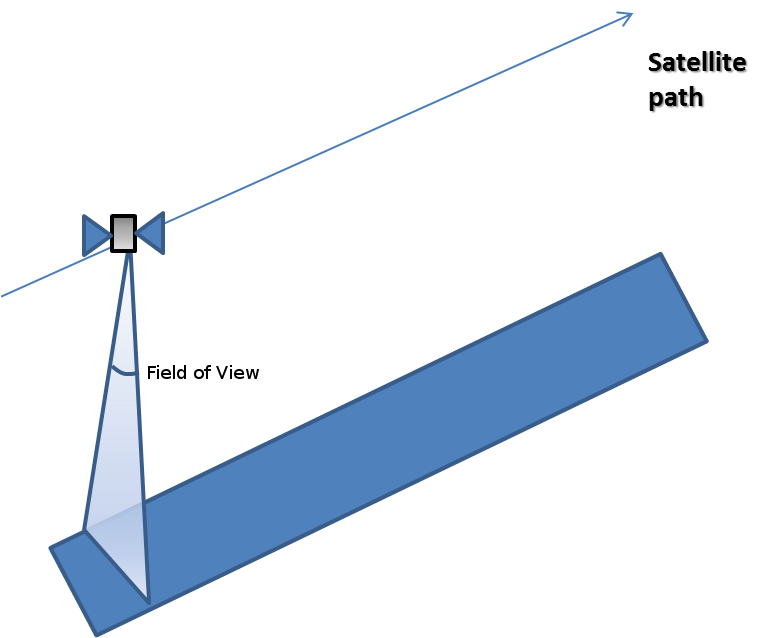
\includegraphics[width=0.6\textwidth]{spaceSystemSimulator/strip-imaging.png}
\caption{Example of strip imaging}
\label{fig:sss-example-strip}
\end{center}
\end{figure}

In the next subsection the assumptions that were made to simulate the system as realistically as possible are described for the scenarios. Note that scenarios 5 and 6 have the same \emph{AOI}, which is the whole land mass on Earth. This involves that because of the huge amount of data that has to be recorded, specific assumptions to the scenarios 5 and 6 were made according to the Fed4FIRE testbeds’ limitations.

\subsubsection{Assumptions in satellite image acquisition}
\label{subsubsec:assumptions}

The \emph{AOI} in each scenario can be acquired by one or more satellites depending on
the size of the \emph{AOI} relatively to the scene size (note that the GEO-Cloud
satellites have a swath of $160km$, thus we divide the acquisition into scenes of
$160km x 160km$). 
In each scenario we call \emph{main satellites} to the satellites with the task
of acquiring the \emph{AOI} (note that all satellites are \emph{main satellites} in the
model for the scenarios 5 and 6). 
Along the duration of the scenario other satellites acquire images of the areas of the Earth surface they are passing over. Those images are not in the area of interest. During the experiments in \bonfire, they will be processed but not stored into the system, since the focus of the mission in every scenario has to be in the defined area of interest. Those non \emph{AOI} images allow us to emulate a real system, since we take into account all the possible inputs to the system (note that in the scenarios 5 and 6 all the images created are \emph{AOI}).

\begin{figure}[!h]
\begin{center}
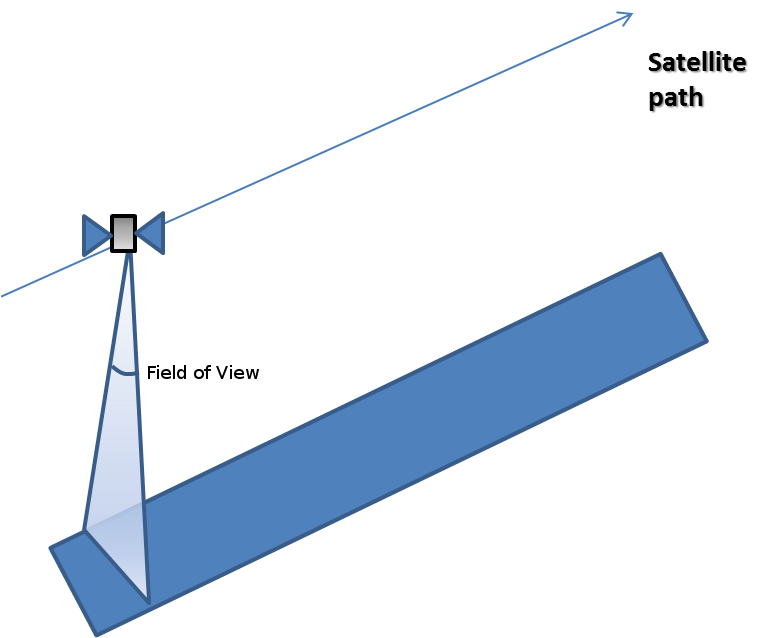
\includegraphics[width=0.6\textwidth]{spaceSystemSimulator/strip-imaging.png}
\caption{Example of strip imaging}
\label{fig:sss-acquisition-diagram}
\end{center}
\end{figure}

Thus, those Non \emph{AOI} images, during the simulation will be acquired,
downloaded to the ground stations, transferred to the cloud and processed, but
not stored, neither catalogued. In addition, it has to be taken into account
that the main satellites can also acquire some images out of the \emph{AOI}
during the duration of each scenario. Those acquired images are also considered
Non \emph{AOI} images. 

In every scenario the time is set to 0 when the simulation starts in the Fed4FIRE environment.

These assumptions are summarized as follows:
\begin{enumerate}
\item Only the scenes acquired by a satellite that include the \emph{AOI} are considered to carry out the complete simulation.
\item Images taken by the satellites that are out of the \emph{AOI} are processed but
  not stored into the system to adjust the experiment execution to the resources
  provided by \bonfire.
\end{enumerate}

\subsubsection{Types of acquisition of the AOI by a single satellite}
\label{subsubsec:types-acquisition}

Depending on the relative sizes of both the \emph{AOI} and the scenes, three different
situations can occur when a single satellite is acquiring images:
\begin{enumerate}
\item Simple acquisition: the \emph{AOI} (at least the part to be imaged by the
  satellite) fits into just one scene.

\begin{figure}[!h]
\begin{center}

\includegraphics[width=0.6\textwidth]{spaceSystemSimulator/simple-acquisition.png}
\caption{Simple acquisition}
\label{fig:sss-simple-acquisition}
\end{center}
\end{figure}
\item Multiple consecutive acquisitions: the \emph{AOI} to be acquired by a satellite
fits in a strip with several scenes.
\begin{figure}[!h]
\begin{center}
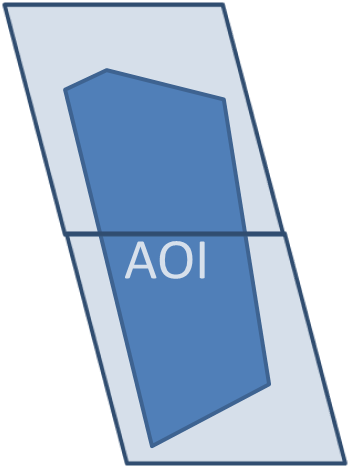
\includegraphics[width=0.6\textwidth]{spaceSystemSimulator/multiple-consecutive-acquisitions.png}
\caption{Multiple consecutive acquisitions}
\label{fig:sss-multiple-acquisition-diagram}
\end{center}
\end{figure}

\item Multiple non-consecutive acquisitions: the \emph{AOI} to be acquired by a
  satellite fits in a strip but there are some scenes between the acquisitions
  that have to be acquired in order to complete the general mission (world map
  daily) but it is not necessary for the scenario.

\begin{figure}[!h]
\begin{center}
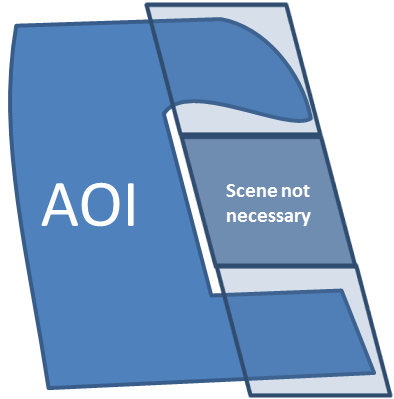
\includegraphics[width=0.6\textwidth]{spaceSystemSimulator/non-consecutive-acquisitions.png}
\caption{Multiple non-consecutive acquisitions}
\label{fig:sss-non-consecutive-acquisition}
\end{center}
\end{figure}

\end{enumerate}


\subsubsection{Parameters required for the simulation of the scenarios}



\begin{equation} \label{eq:solve}
x^2 - 5 x + 6 = 0
\end{equation}



\subsection{Image Downloading}
\label{subsec:image-downloading}

The acquired images by the satellites shall be downloaded to the emulated ground
stations through the antennas network designed <<(see GEO-Cloud-D10.8-Detailed
design report-2014-01-31)>>. All the scenarios finish at $T_f$, when the last
main satellite completely downloads the last acquired portion of the
\emph{AOI}. During the simulation, the rest of the satellites not overflying the
\emph{AOI} would be imaging other places; these images will also be downloaded
and processed in parallel to the \emph{AOI} images to simulate a realistic case,
but as previously explained those images will not be stored nor catalogued.

Because of the limitations in the testbeds (limited storage and compute
resources in \bonfire cloud and multiplexed channel over virtual networks in
\vw) it is necessary to scale the data involved in these simulations from the
original design of the GEO-Cloud experiment. It has been decided to change the
designed compression rate from lossless compression $2:1$ to a rate compression
$14:1$. With this change, the data volume has been reduced and the size of every
$160km x 160km$ scene after compression is now $288MB$ instead of the almost
$2GB$ size of the original images.

In order to download the data, the satellites have to be inside the visibility cone of a ground station. During these accesses, the satellites download images at a rate of $160Mbps$. Part of these images are in memory before entering the visibility cone and others are being acquired simultaneously during the downloading task <<(see section 2.3 for a wider explanation of the download parameters and Figure \ref{fig:sss-multiplexed-downloading}).>>

\begin{figure}[!h]
\begin{center}
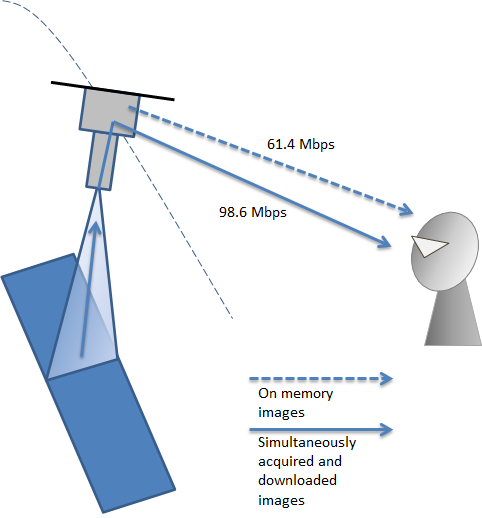
\includegraphics[width=0.6\textwidth]{spaceSystemSimulator/multiplexed-downloading.png}
\caption{Multiplexed images downloading}
\label{fig:sss-multiplexed-downloading}
\end{center}
\end{figure}



It is possible that the duration of the accesses and the time to download an image are not multiples of $T_scene=23.4s$. In this case, an image would be partially downloaded at the end of the access but it would be supposed that this image is completely downloaded in the following access in other ground station. 

For the memory management, a \emph{LIFO} (last in, first out) procedure is
applied. This implies that the latest acquired images will be downloaded as soon
as possible. This imposes that when a satellite is inside the visibility cone of
a ground station both the images latest acquired and the images that are being
acquired of the \emph{AOI} will be simultaneously downloaded by multiplexing
them. Note that because of differences between the rate of acquisition and
downloading, and also because of the compression process, the downloading of
images that are being simultaneously acquired do not occupy all the bandwidth of
$160Mbps$; the portion not occupied is used to download on board storage also
with a \emph{LIFO} process (See 2.3 numbers 3 to 5).


As an example, the data of the accesses for the Scenario 2 are included in the
following table:


\begin{table}[hp]
  \centering
  {\small
  
\begin{tabular}{p{.2\textwidth}p{.2\textwidth}c c c}\hline
\tabheadformat
\tabhead{Sat. Ident. Number} & \tabhead{Ground Station} &
\tabhead{Access Start Time} & \tabhead{Access Stop Time}
&\tabhead{Duration of the passes}\\
\tabheadformat
 & &$(s)$ &$(s)$ &$(s)$ \\\hline
        1 & Krugersdorp  & 54184.2 &54516 &331.8\\\hline
        2 & Dubai        & 54184.2 &54516 &331.8\\\hline
        2 & Krugersdorp  & 54549.4&54753.4 &204\\\hline
        3 & Dubai        & 54060 &54753.4&204\\\hline
        4 & Dubai        &54060&54337.5&277.5\\\hline              
        4 & Svalvard     &54660&54753.4&93.4\\\hline
        5 & Svalvard     &54316.3&54753.4&437.1\\\hline
        6 & Prince Albert&54708.1&54753.4&45.3\\\hline
        6 & Svalvard     &54060&54639.4&579.4\\\hline
        7 & Prince Albert&54362&54753.4&391.4\\\hline
        7 & Svalvard     &54060&54296.7&236.7\\\hline
        8 & Prince Albert&54060&54577.9&517.9\\\hline
        9 & Prince Albert&54060&54246.8&186.8\\\hline
        15 & Troll       &54419&54670.3&251.3\\\hline
        16 & Troll       &54085.6&54303.4&217.8\\\hline
        17 &Krugersdorp  &54495.4&54753.4&258\\\hline              
\end{tabular}

  }
  \caption{Example of data of accesses for Scenario 2}
  \label{table:sss-accesses-scenario2}
\end{table}


Next, a summary of the assumptions made for the image downloading from the
satellites to the ground stations are described:
\begin{enumerate}
\item Time to process the images on board before downloading is considered to be instantaneous. Then, the simultaneous acquisition and download of the AOI inside the visibility cone is done without latency.
\item The ground stations network was designed to guarantee the download of a complete world map in a daily basis. With this assumption into account, the management of the memory on board of each satellite does not require an additional design. This involves that we do not know in which ground station all the areas acquired out of a visibility cone are downloaded. 
\item Because of the small gap between the satellites, which are in the same orbit, more than one antenna in each ground station is required to be available. This provides the possibility of having simultaneous contacts with all the satellites inside the visibility cone.
\end{enumerate}

\subsection{Getting the satellite data}
\label{subsec:getting-satellite-data}

The steps to obtain and simulate the realistic behaviour of the satellites are
next described. 


\subsubsection{Extraction of the real behaviour of the satellite constellation
  in the scenarios}
\label{subsubsec:extraction}

The first point is to obtain the realistic behaviour of the constellation of satellites designed in “GEO-Cloud-D10.8-Detailed design report-2014-01-31.docx”.  For that purpose, the constellation of satellites and the ground stations were implemented in the Systems Tool Kit® (STK) software.

The next steps were followed to obtain the values of the parameters required for the simulations of the defined scenarios:
\begin{itemize}
\item Commonly for all the scenarios:
\begin{enumerate}
\item Implementation of the satellite constellation.
\item Implementation of the ground station network.
\item Calculation of the access time for each satellite communicating with each
  ground station during 24 hours.
\newcounter{enumTemp}
\setcounter{enumTemp}{\theenumi}
\end{enumerate}
\item For each different scenario:
\begin{enumerate}
\setcounter{enumi}{\theenumTemp}
\item Identification of the main satellites.
\item Extraction of the times each satellite is acquiring the AOI: $[T_AOI]_0i$ and $[T_AOI]_fi$.
\item Calculation of the number of scenes acquired: n.
\item Extraction of the access duration of each satellite with the ground stations it communicates within the scenario duration: $[T_GS]_0ij$ and $[T_GS]_fij$.
\item Start time of the scenario: $T_0$.
\item End time of the scenario: $T_f$.
\end{enumerate}
\end{itemize}

\subsubsection{Exportation of data to the simulator}

Once obtained the previous data, it is exported to different ``CSV'' format files: 

\begin{itemize}
\item 	The \emph{Scenario\_<NUM>\_<SCENE>.csv} files: it contains the information
  of the $[T_GS]_0ij$ and $[T_GS]_fij$ for each scenario. \emph{<NUM>} indicates
  the number of the scenario and \emph{<SCENE>} the name of the scenario. In the
  GEO-Cloud experiment we simulate 6 scenarios. The previous parameters are
  defined in the following table:


For example, the format of the resulting \emph{Scenario\_1\_
Emergencies\_Lorca\_Earthquake.csv} file with the $[T_GS]_0ij$ and $[T_GS]_fij$
information for the Lorca scenario, looks like the code extract shown in Listing
\ref{code:sss-info-scenario}.
\lstset{%
  backgroundcolor = \color{gray95},
  rulesepcolor    = \color{black},
}

\begin{listing}[
  float=h!,
  caption  = {Extract of the \emph{Scenario\_1\_Emergencies\_Lorca\_Earthquake.csv}
    of the Lorca scenario},
  label    = code:sss-info-scenario]
"GEO-Cloud_005-To-Troll - Access","Start Time (EpSec)","Start Time (UTCG)","Stop Time (EpSec)","Stop Time (UTCG)","Duration (sec)"
1,63638.000,11 Aug 2014 10:10:38.000,63661.400,11 Aug 2014 10:11:01.400,23.400

"GEO-Cloud_006-To-Troll - Access","Start Time (EpSec)","Start Time (UTCG)","Stop Time (EpSec)","Stop Time (UTCG)","Duration (sec)"
7,63638.000,11 Aug 2014 10:10:38.000,63661.400,11 Aug 2014 10:11:01

\end{listing}

In the code, a heading is separated into columns. It is divided as follows: 


\begin{table}[hp]
  \centering
  {\small
  


\begin{tabular}{p{.2\textwidth}p{.2\textwidth}}
  \tabheadformat
  \tabhead{Column Title}   &
  \tabhead{Function}\\
\hline
\textit{GEO-Cloud\_sat-To-station}         & Represents the access of a satellite to the specific ground station. sat represents the satellite number and station the ground station name. \\
\hline
\textit{Start Time (EpSec)}         & Means $[T_{GS}]_{0ij}$. \\
\hline
\textit{Start Time (UTCG)}         & Means  $[T_{GS}]_{0ij}$ in UTCG format \\
\hline
\textit{Stop Time (EpSec)}         & Means $[T_{GS}]_{fij}$ \\
\hline
\textit{Stop Time (UTCG)}         & Means $[T_{GS}]_{fij}$ in UTCG format. \\
\hline
\textit{Duration (sec)}         & Means $[\Delta T_{GS}]_{ij}$. \\
\hline
\end{tabular}


% Local variables:
%   coding: utf-8
%   ispell-local-dictionary: "castellano8"
%   TeX-master: "main.tex"
% End:

  }
  \caption{Columns headings \emph{Scenario\_<NUM>\_<SCENE>.csv} files}
  \label{table:sss-headings-scenario2}
\end{table}

\item 	The \emph{All\_Scenarios.csv} file: it contains the information of the $[T_AOI]_0i$ and $[T_AOI]_fi$ for all the scenarios.
A piece of the \emph{All\_Scenarios.csv} file that contains the $[T_AOI]_0i$ and $[T_AOI]_fi$ of all the scenarios is shown in Listing \ref{code:sss-all-scenarios}.  It also contains  $T_0$ ,$T_f$ and the number $n$ of \emph{AOI} obtained images.


\begin{listing}[
  float=h!,
  caption  = {Extract of the \emph{All\_Scenarios.csv} code of the Lorca scenario},
  label    = code:sss-all-scenarios]

Scenario,Start Sce,End Sce,Sat,Start sat,End Sat,Images
1,63638,63661.4,11,63638,63661.4,1
,,,,,,
2,54060,54753.4,4,54060,54083.4,1
,,,3,54390,54413.4,1
,,,2,54730,54753.4,1
,,,,,,
3,62480,63865.4,15,62480,62503.4,1
,,,14,62821,62844.4,1
,,,13,63161,63184.4,1
,,,12,63501,63524.4,1
,,,11,63842,63865.4,1
\end{listing}

This file was manually computed. The required fields to describe the behaviour of the satellites acquiring the \emph{AOI} are the following:

\begin{table}[hp]
  \centering
  {\small
  


\begin{tabular}{p{.2\textwidth}p{.2\textwidth}}
  \tabheadformat
  \tabhead{Column Title}   &
  \tabhead{Function}\\
\hline
\textit{Scenario}         & Scenario number. Indicates the scenario executed \\
\hline
\textit{Start Sce}         & Indicates the start of the scenario. It is $T_0$  \\
\hline
\textit{End Scen}         &Indicates when the scenario finishes. It is $T_f$ \\
\hline
\textit{Sat}         & Indicates the number of the \emph{main satellite}.\\
\hline
\textit{Star Sat}         & The time when the satellite starts acquiring the \emph{AOI}. It is $[T_{AOI}]_{0i}$. \\
\hline
\textit{End Sat}         & The time when the satellite finishes acquiring the \emph{AOI}. It is $[T_{AOI}]_{fi}$ \\
\hline
\textit{Images}         & This is the number of \emph{AOI} images. It is $n$.\\
\hline
\end{tabular}


% Local variables:
%   coding: utf-8
%   ispell-local-dictionary: "castellano8"
%   TeX-master: "main.tex"
% End:

  }
  \caption{Columns headings of the \emph{All\_Scenarios.csv} file}
  \label{table:sss-all-scenarios}
\end{table}

\end{itemize}


\subsubsection{Processing of the Scenario\_<NUM>\_<SCENE>.csv and
 All\_Scenarios.csv}
\label{subsubsec:processing-files}

A script is designed and developed to get and merge the data from the \emph{Scenario\_<NUM>\_<SCENE>.csv} and the \emph{All\_Scenarios.csv} files, and to store the information in the database:  \emph{setDatabase.py}. It was developed in Python 2.7 but it is also compatible with all Python versions.

This has to be done because as previously explained
\emph{Scenario\_<NUM>\_<SCENE>.csv} contains the $[T_GS]_0ij$ and $[T_GS]_fij$
parameters of each single scenario and \emph{All\_Scenarios.csv} the
$[T_AOI]_0i$ and $[T_AOI]_fi$ of all the scenarios. Thus the script matches the
$[T_GS]_0ij$ and $[T_GS]_fij$ of one scenario with the $[T_AOI]_0i$ and $[T_AOI]_fi$ of such a scenario.

To execute \emph{setDatabase.py} the arguments depicted in Table \ref{table:sss-arguments-setdabatase}are required.
\begin{table}[hp]
  \centering
  {\small
  


\begin{tabular}{p{.2\textwidth}p{.2\textwidth}}
  \tabheadformat
  \tabhead{Argument Position}   &
  \tabhead{Meaning}\\
\hline
\textit{1}         & IP direction of the host which contains the MySQL database\\
\hline
\textit{2}         & The relative path or absolute path of the file that contains the information of all scenarios (see Listing \ref{code:sss-all-scenarios})
  \\
\hline
\textit{3\ldots}         &The \emph{Scenario\_<NUM>\_<SCENE>.csv} files that contain the events occurred in a particular scenario. At least one file must be introduced, otherwise an execution error is produced. \\\hline
\end{tabular}


% Local variables:
%   coding: utf-8
%   ispell-local-dictionary: "castellano8"
%   TeX-master: "main.tex"
% End:

  }
  \caption{Arguments of \emph{setDatabase.py}}
  \label{table:sss-arguments-setdatabase}
\end{table}

An example of the execution of the programme is the following:
\begin{itemize}
\item python setDatabase.py 192.168.0.2 All\_scenarios\_file.csv Scenario\_1\_Example1.csv Scenario\_2\_Example2.csv Scenario\_3\_Example3.csv
\end{itemize}


\subsection{Space System Simulator}

The \sss is constituted by the following modules:
\begin{itemize}
\item The Database
\item The \satss
\item The \gsss
\end{itemize}


To simulate every scenario, on the one hand, the \satss is executed. It is
constituted by 17 \emph{Satellite Simulators} of individual satellites; each one
reproduces the characteristic behaviour of every single satellite in the
constellation.
On the other hand the \gsss is also executed. As in the case of the \satss, the
\gsss is constituted of 12 \emph{Ground Station Simulators} of individual ground
stations reproducing the behaviour of every single ground station of the
designed network. 
The diagram in Figure \ref{fig:sss-sss-architecture} depicts a scheme
representing the \sss.

\begin{figure}[!h]
\begin{center}
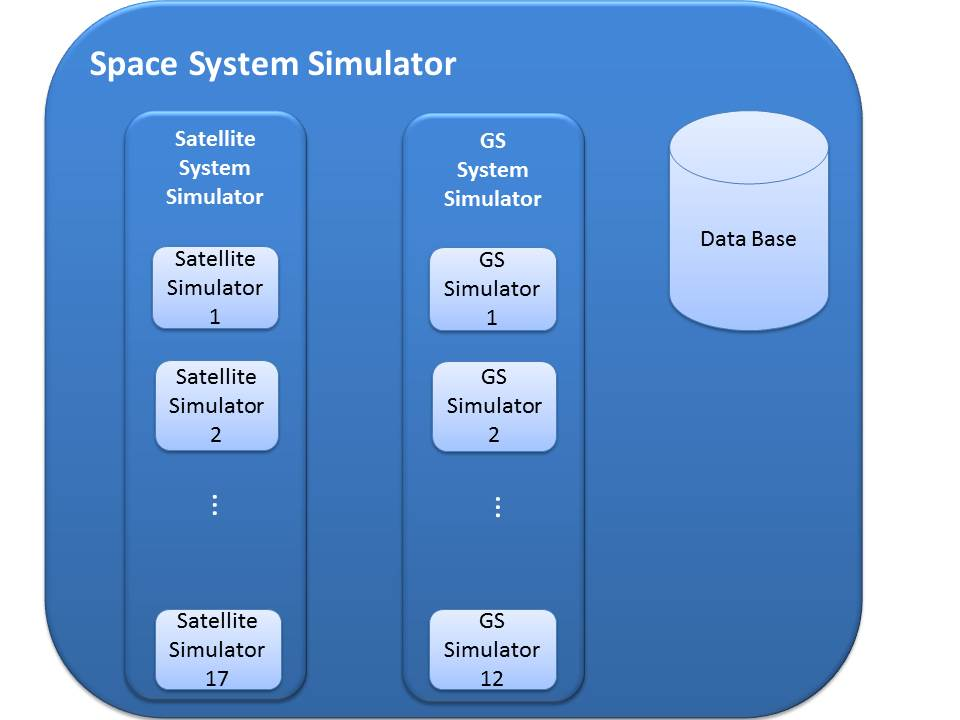
\includegraphics[width=0.6\textwidth]{spaceSystemSimulator/sss-architecture.jpg}
\caption{Space System Simulator's Architecture}
\label{fig:sss-architecture}
\end{center}
\end{figure}

The Space System Simulator sequentially follows the next steps during the
execution:
\begin{itemize}

\item First, \emph{setDatabase.py} is executed. The script fills the database fields with the information of every scenario.
\item Second, the \gsss is executed. The \gsss can execute all the \emph{Ground Station Simulators} or some of them individually to simulate faults in the ground stations as it can occur in reality. Thus, when a satellite needs to download data into a ground station that is offline, it will receive an exception so the downloading of images does not start.
\item Third, the \satss is executed. As in the previous case, the \satss can execute all the \emph{Satellites Simulators} or some of them individually for the same reason. 
\item Finally, when the scenario finishes, the simulation is stopped.
\end{itemize}
The \emph{Database}, the \satss and the \gsss are thoroughly described in the
next subsections. 

\subsubsection{Database}

A database containing all the required data for the simulations was
implemented. The selected database management system (DBMS) is MySQL. It was
selected because it is friendly usable, works in multiple platforms, provides
transactional and nontransactional storage engines and the server is a separate program for use in a client/server networked environment. 

The design of the database architecture is shown in Figure 10

\begin{figure}[!h]
\begin{center}
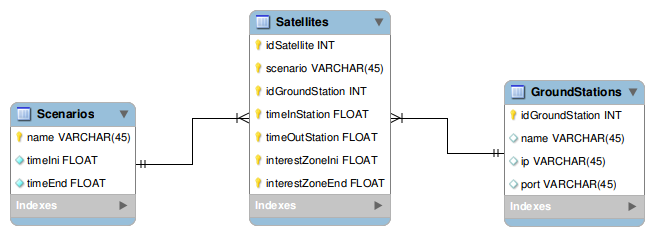
\includegraphics[width=0.6\textwidth]{spaceSystemSimulator/database-architecture.png}
\caption{Database architecture}
\label{fig:sss-database-architecture}
\end{center}
\end{figure}

The database is constituted by three tables: Scenarios table, Satellites table
and GroundStations table. The functionalities of the tables are described in
Table 7:


tablas


\subsubsection{Database Filling}

\begin{itemize}

\item \textbf{Filling during initialization}

The database is filled during the initialization process by executing
\emph{setDatabase.py} as previously described in Section
\ref{subsubsec:processing-files}. This execution makes the following sequential
actions:
\begin{enumerate}
\item All the data that is in the database is cleaned to avoid inconsistencies.
\item The \emph{GroundStation} table is filled with the ground stations information (only name and id).
\item The Scenario table is completely filled with the data of each scenario.
\item Finally, the Satellites table is completely filled. This process joins the
  information contained in the \emph{Scenario\_<NUM>\_<SCENE>.csv} with file
  \emph{All\_Scenarios.csv}. This means that for each Scenario the $[T_GS]_0ij$,
  $[T_GS]_fij$,  $[T_AOI]_0i$ and $[T_AOI]_fi$ representative of the simulated
  scenario are taken. That information is inserted into the database as follows: 
\begin{itemize}
\item For each scenario the information regarding the accesses of the satellites to the ground stations are selected, $[T_GS]_0ij$ and $[T_GS]_fij$. 
\item Those accesses are merged with the \emph{All\_scenarios.csv} file in order to obtain the accesses of the satellites in which there are \emph{AOI} images. 
\item Then if the satellite acquired an \emph{AOI} in the current scenario, the information of the \emph{AOI} is also included in the database. 
\item Otherwise the fields with the information regarding the \emph{AOI} are filled
  with $-1$ value. 
\end{itemize}
\end{enumerate}

\item \textbf{Filling during the execution of the Space System Simulator}

During the execution of the \gsss the ip and port columns in the
\emph{GroundStations} table are filled. This is done when a \emph{Ground Station
  Simulator} starts its execution in a node. The \emph{IP adress} and
\emph{port} of that node are obtained and included in the database. Once each
ground station has an \emph{IP adress} and a \emph{port} associated, the \emph{Satellite Simulators} can read both of them and communicate with \emph{Ground Stations Simulators} servers.

\end{itemize}


\subsection{Satellite System Simulator}

The \satss reproduces the behaviour of the 17 satellites constellation by executing 17 individual \emph{Satellite Simulators} characterized by the specific behaviour of each satellite. 

The \satss is a manager that executes 17 \emph{Satellite Simulators}. The
\emph{Satellite System Simulator} requires the scenario number and the \emph{IP adress} of the database as an input and executes the \emph{Satellite Simulators} by providing them the specific identity of the satellite \emph{(idSatellite)}, number of the scenario \emph{(S)} and IP of the distributed database  \emph{(ipDatabase)}.

Next, the architecture of the \emph{Satellite Simulator} for each individual
satellite is described.

